\documentclass[11pt]{article}
\usepackage[letterpaper]{geometry}
\usepackage{times}
\usepackage{verbatim}
\usepackage{graphicx}
\usepackage{float}
\usepackage{fullwidth}
\usepackage{amsmath}
\usepackage{amssymb}
\usepackage{hyperref}
\graphicspath{{Images/}}
\title{ENGR-241 Transfer Function Lab}
\author{Jeremy Munson, Lauren Speirs \& Andrew Henrikson}
\geometry{top=.8in, bottom=.8in, left=.8in, right=.8in}

\setlength{\parindent}{0em}
\setlength{\parskip}{.5em}
\begin{document}
	\maketitle
	\subsection*{Overview}
	For this lab we calculated the transfer function then built the required circuit from the lab guidelines. We then calculated the voltage across the capacitor and compared our results from our circuits output to the oscilloscope. We then built the circuit using Orcad and analyzed the ciruit using the Laplace function in Pspice and compared its output to our previous results.
		\subsection*{Circuit Diagrams}
		Our suggested values and measured values for our components used are shown in the table below. The percent error is also listed.
		\begin{table}[h]
		\def\arraystretch{1.2}%
		\begin{tabular}{|l|l|l|l|}
			\hline
			Components       	& Suggested 		& Measured      	&\% Diff	\\ \hline
			Resistor 1   		& $1 k\Omega$		& $0.998 k\Omega$   & 2\%	     \\ \hline	
			Resistor 2			& $240 \Omega$		& $241 \Omega$      & 0.4\%       \\ \hline
			Inductor			& $220\mu H$		& $199\mu H$		& 10.6\%		\\ \hline
			Capacitor			& $1 \mu F$			& $0.95 \mu F$		&5.3\%		\\ \hline
		\end{tabular}
	\end{table}
	
	\begin{figure}[H]
		\centering
		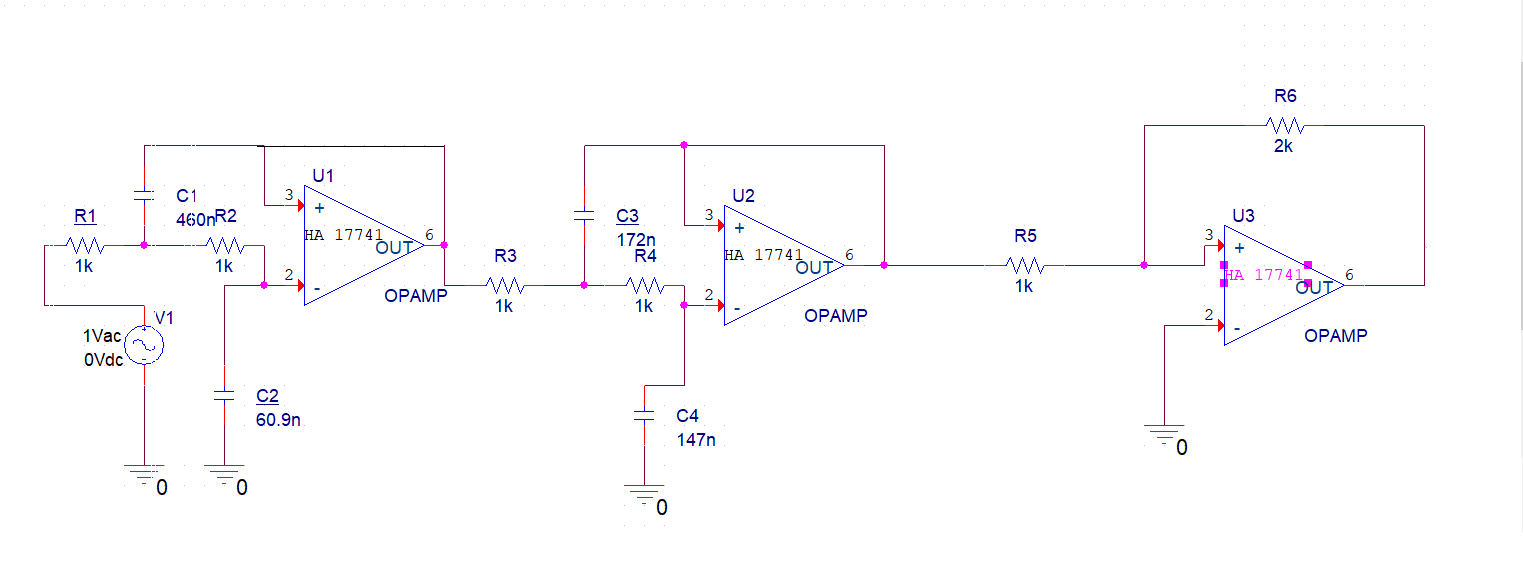
\includegraphics[width=5in]{images/diagram.png}
	\end{figure}
	
	
	\subsection*{Calculations}
	
\end{document}
